\chapter{Extensions}

\section{The Introduction of Evidence} \label{sect:evidence}

In many studies of multi-agent communication, there exists a ``true state'' of the world that the agents must agree upon. Here, we will explore the effects of including such a state as well as evidence in support of it. We arbitrarily assign one state of the world to be ``true''. At each iteration, a subset of the population is selected to receive evidence. This is done by conducting $K$ Bernoulli trials, with probability $\pi$. There is also a chance $c$ that the evidence is accurate. This can be thought of as an agent querying an external, fallible oracle. Here, the oracle returns a singleton set, containing a single element that is only partially accurate. This assertion is then incorporated into the agent's beliefs as in~\cref{eq:BU_update_rule}

It is expected that the introduction of this evidence will sway the agents toward the true state of the world when $c > \frac{1}{n}, \pi > 0$, an expectation supported by~\cref{fig:evidence}. In this figure, the true state of the world is rotated on the $2,000^{\textnormal{th}},5,000^{\textnormal{th}},10,000^{\textnormal{th}} $ and $ 20,000^{\textnormal{th}}$ iterations. \cref{fig:evidence_deviation} shows the average J-Divergence between the true state of the world and each agent at each time step, referred to as the deviation. 


\begin{figure}[H]
 \centering
  \begin{subfigure}[ht]{0.45\textwidth}
    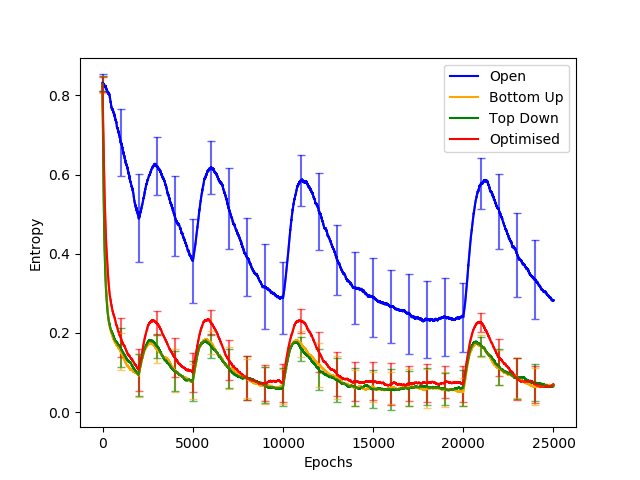
\includegraphics[width=\textwidth]{Images/Figures/Evidence/EntropyGood.png}
    \caption{Entropy}
 \end{subfigure}
 \hfill
 \begin{subfigure}[ht]{0.45\textwidth}
    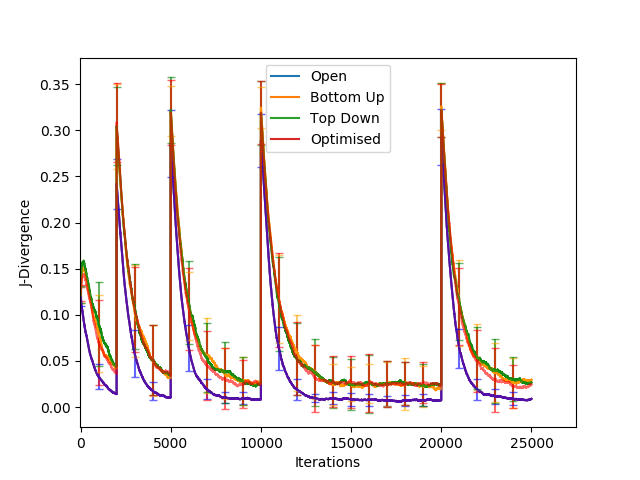
\includegraphics[width=\textwidth]{Images/Figures/Evidence/J-DivGood.png}
    \caption{Deviation} \label{fig:evidence_deviation}
 \end{subfigure}
 \caption{Two plots to show the change in entropy and deviation from the true state over time, for the Open, Bottom Up, Top Down, and Optimised models. These plots were obtained using Passive listeners, and were averaged over $100$ runs. Here, $\pi = 0.001, c=0.9$. At the $2,000^{\textnormal{th}},5,000^{\textnormal{th}},10,000^{\textnormal{th}} $ and $ 20,000^{\textnormal{th}} $, the true state of the world $H_j$ is switched to be $H_{j+1}$, highlighted by the jumps in deviation between the true state and each agent.}\label{fig:evidence}
\end{figure}

It can be clearly seen that the entropy in the Open model is significantly higher than the rest of the models. Recalling the results of~\cref{sect:analysis}, this is not unexpected. The agents in the Open model cluster together, forming a group in the centre of the simplex. With probability $\pi$, an agent is selected to receive evidence, therefore leaving the main group. Each time such an agent is selected as speaker while outside the group, the centroid of the population moves toward it. When both $\pi$ and $c$ are sufficiently large, this moves the entire population toward the true state. It is apparent that the Open model has the smallest deviation of any of the models, as shown in~\cref{fig:evidence_deviation}. The other three models behave similarly in these plots. At first sight, this does not seem to make sense in conjunction with the highest entropy value on the plot. However, agents in the other three models have a tendency to lie along the edges of the simplex, for which entropy values are low, whereas the Open model rarely reaches these extremities. Instead, agents in the Open model move cohesively in the direction of the true state, getting all the agents close, yielding a small deviation. Conversely, the other models achieve large numbers of agents with strong beliefs in a subset of the possible worlds, that are not as close to the true state as the Open model. 

Another factor in favour of the Open model in this paradigm is that the magnitude of its updates is much smaller than the other models. Consider an agent $x$, such that $\underline{\mathbf{P}}^t_x = [0.4, 0.6, 0]^T$. This agent is undecided between two states, with a slight preference for $H_2$. In this example, let the rest of the population be almost certain in the true state, $H_1$. If $x$ is selected as speaker in the Bottom Up, Top Down, or Optimised model, it is likely that it will assert $\mathbf{A} = \{ H_2 \}$. In this case, the listener agent will update $\approx \alpha$ toward $H_2$, as in~\cref{fig:sierpinski_triangle_intro}. However, if $x$ is an Open agent, it broadcasts its beliefs, causing the listener to update only $\approx \frac{\alpha}{2}$ toward $H_2$. This means that the Open model is slightly slower to react, but much more robust to changes, inexorably updating toward the true state.  

When the true state of the world is rotated, all models recover, with the agents quickly re-converging to the true state. This change in the true state corresponds with the vertical sections of~\cref{fig:evidence_deviation}. This recovery is only possible for agents that have not reached certainty in a single state. Once an agent's beliefs $\underline{\mathbf{P}}_x^t = [1,0,0]^T$, it is impossible to persuade them to alter their opinions. In simulation, this the true state to remain the same for many thousands of iterations, depending on $\pi$ and $c$. 


\section{Method for the Reconstruction of an Agent's Beliefs}

In this Optimised model, it is assumed that the agents have access to perfect information about the nature of the listener's beliefs before they make an assertion. In this model, the speaker creates the argument that will cause the listener to update their beliefs to be as close as possible to the speaker. The complete understanding of the way in which the listener will react is highly unrealistic, as it is rare that any agent would be so open or predictable. To weaken this assumption it is possible to reconstruct the listener's beliefs based on their previous assertions as speaker.

Let each agent in the population keep a record of the last $\zeta$ assertions that each speaker has made in the set $\mathbf{A}_\zeta$. It is likely that the average of these assertions will reflect an agent's underlying set of beliefs. Hence, the speaker takes an average of the last $\zeta$ assertions by the listener to approximate their beliefs at the current time step, re-normalising it to be a probability distribution. This approximation takes the form

\begin{equation} \label{eq:reconstructive}
    \hat{p}_{l,j} = \frac{\abs{ \{H_j: H_j \in \mathbf{A}_\zeta \} } }{ \sum_k^n \abs{ \{ H_k; H_k \in \mathbf{A}_\zeta \} }   }.
\end{equation}

\Cref{fig:reconstructive} shows a comparison between the standard Optimised model with perfect information and with reconstructed information. 


\begin{figure}[H]
 \centering
  \begin{subfigure}[ht]{0.45\textwidth}
    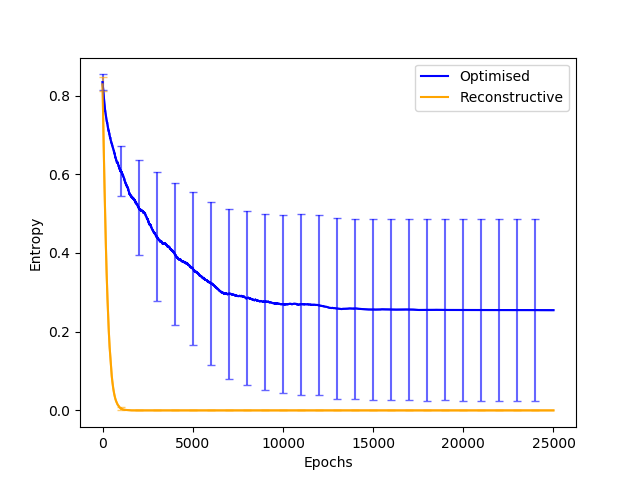
\includegraphics[width=\textwidth]{Images/Figures/Reconstructive/Entropy_reconstruct_better.png}
    \caption{Entropy}
 \end{subfigure}
 \hfill
 \begin{subfigure}[ht]{0.45\textwidth}
    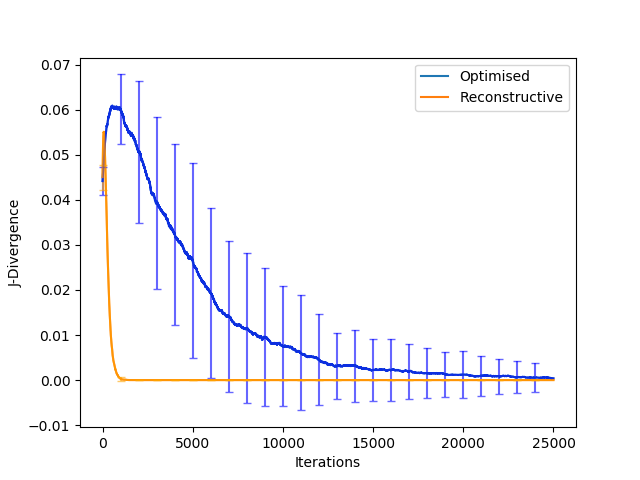
\includegraphics[width=\textwidth]{Images/Figures/Reconstructive/J-Div_reconstruct_better.png}
    \caption{J-Divergence}
 \end{subfigure}
 \caption{Two plots to show the change in entropy and J-Divergence over time, for the Optimised model with perfect information and reconstructed information at $\zeta = 10$. These plots were obtained using Passive listeners, and were averaged over $100$ runs.}\label{fig:reconstructive}
\end{figure}

This shows that the reconstructive model almost immediately achieves a consensus in a single state of the world. This behaviour is highly consistent, as shown by the narrow error bars. However, the Optimised model with perfect information again underperforms. The J-Divergence decreases to $0$ suggesting that the agents do reach a consensus, however, the consensus appears to be in an uncertain distribution. It is likely that the width of the error bars in the entropy plot is due to the Optimised model again converging to a vertex in one of the sub-triangles of~\cref{fig:chaos_game}. 

It is interesting to note that the error between the listener's beliefs and the speaker's approximation decreases to $0$. This is intuitive, as once an agent is highly confident in a single state, it will likely assert that single state alone. Thus the approximation will become based on the repeated assertion of a single state, decreasing to $0$ as the system converges. 

These results show that the Optimised model is an insufficient method for achieving consensus with perfect information, however, with approximate information, it quickly converges to a certain consensus. 



\section{Mixed Population Tests} \label{sect:pop_tests}

In Economics, agents can be assigned a variety of different trading strategies, with the aim of making deals that maximise the agent's profit. The earliest strategies proposed were rudimentary, such as ZI-U and ZI-C~\cite{Gode1993AllocativeRationality}, with later models incorporating machine learning techniques to improve their performance, such as ZI-P, GDX and AA~\cite{Cliff1997Minimal-IntelligenceEnvironments, Gjerstad1998PriceAuctions, Vytelingum2006TheAuction}. \cite{Vach2015ComparisonAgents} provides an excellent comparison of the performance of these strategies when tested against each other in various concentrations. This analysis inspires the following analysis. In order to determine the most persuasive argumentation strategy, two different speaker models can be included in the same population. A record is kept of the change in J-Divergence that is attributed to arguments created by both models, and the ``victor'' is the model that accounts for the greatest change in J-Divergence after $5,000$ iterations. Furthermore, different concentrations of each strategy should be considered, as, in Vach's work, some strategies perform best when in a minority. 

The following table shows the mean and standard deviation of the J-Divergence, summed for the model of each speaker across $5,000$ iterations for a population of $100$ agents mixed to the corresponding concentrations. It also shows the fraction of those $1,000$ runs that was ``won'' by each strategy. The victors are shown in bold. It is important to note that these experiments assume each interaction between a speaker and listener to be independent, such that the order in which agents attempt to persuade each other is unimportant. This is the ``well-stirred'' assumption~\cite{Parker2009CooperativeProblem}. 

\begin{table}[H]
\begin{adjustbox}{max width = \textwidth}
\begin{tabular}{ll||cc|cc|cc|cc|cc|cc}
 &  & Open & Bottom Up & Open & Top Down & Open & Optimised & Bottom Up & Top Down & Bottom Up & Optimised & Top Down & Optimised \\ \hline \hline
\multirow{3}{*}{1:5} & Wins & 0 & \textbf{1000} & 0 & \textbf{1000} & 0 & \textbf{1000} & 0 & \textbf{1000} & 0 & \textbf{1000} & 0 & \textbf{1000} \\
 & Mean & 102.62 & 556.77 & 266.24 & 310.25 & 32.71 & 461.35 & 116.48 & 572.93 & 98.44 & 559.44 & 114.65 & 537.71 \\
 & Standard Deviation & 33.89 & 182.86 & 83.19 & 96.71 & 10.48 & 165.44 & 37.39 & 178.11 & 976.91 & 169.07 & 34.24 & 161.23 \\ \hline
\multirow{3}{*}{2:4} & Wins & 0 & \textbf{1000} & 0 & \textbf{1000} & 0 & \textbf{1000} & 0 & \textbf{1000} & 0 & \textbf{1000} & 0 & \textbf{1000} \\
 & Mean & 195.84 & 434.74 & 196.56 & 439.31 & 63.32 & 301.55 & 237.99 & 465.36 & 197.7 & 459.79 & 235.58 & 573.71 \\
 & Standard Deviation & 62.09 & 138.50 & 61.76 & 136.48 & 21.72 & 118.50 & 71.09 & 178.11 & 65.07 & 138.96 & 34.24 & 131.35 \\ \hline
\multirow{3}{*}{3:3} & Wins & 15 & \textbf{985} & 2 & \textbf{998} & 0 & \textbf{1000} & \textbf{763} & 237 & 0 & \textbf{1000} & 25 & \textbf{975} \\
 & Mean & 259.22 & 298.03 & 268.98 & 313.77 & 91.57 & 191.49 & 340.28 & 328.92 & 300.58 & 357.97 & 345.47 & 377.57 \\
 & Standard Deviation & 87.52 & 101.61 & 86.28 & 100.07 & 33.15 & 76.38 & 110.83 & 106.40 & 100.03 & 104.51 & 106.46 & 102.59 \\ \hline
\multirow{3}{*}{4:2} & Wins & \textbf{1000} & 0 & \textbf{1000} & 0 & \textbf{757} & 243 & \textbf{1000} & 0 & \textbf{997} & 3 & \textbf{1000} & 0 \\
 & Mean & 275.46 & 168.0 & 296.03 & 186.38 & 114.61 & 109.65 & 470.81 & 223.92 & 421.71 & 256.17 & 471.36 & 267.90 \\
 & Standard Deviation & 101.28 & 63.77 & 101.13 & 63.80 & 38.93 & 42.83 & 142.78 & 67.31 & 137.47 & 68.12 & 135.33 & 63.46 \\ \hline
\multirow{3}{*}{5:1} & Wins & \textbf{789} & 211 & \textbf{1000} & 0 & \textbf{1000} & 0 & \textbf{1000} & 0 & \textbf{1000} & 0 & \textbf{1000} & 0 \\
 & Mean & 261.47 & 256.25 & 242.22 & 76.76 & 125.61 & 50.62 & 571.24 & 109.50 & 541.02 & 139.20 & 585.96 & 143.79 \\
 & Standard Deviation & 87.74 & 97.96 & 89.27 & 29.16 & 40.51 & 19.65 & 181.24 & 33.52 & 178.71 & 33.59 & 171.96 & 31.57
\end{tabular}
\end{adjustbox}
\caption{Table to show results of mixing different persuasion strategies together in different concentrations, with Passive listeners. The victor of the majority of the $1,000$ games is shown in bold, alongside the mean and standard deviation J-Divergence each strategy is responsible for. }
\end{table}


The results of this experiment are much as one would expect, showing that, in almost all cases, the agent in the majority is responsible for the most movement in the population. However, there are some cases where a strategy underperforms. For instance, the Open vs Optimised games with a $4:2$ concentration show the Optimised solution winning $24.3 \%$ of the time. This highlights the limitations of the Open model, as demonstrated in~\cref{sect:evidence}, with its more diluted arguments limiting the potency of the argument. Another remarkable observation is the result of the Open vs Bottom Up game with a $5:1$ concentration. This is unexpected and the reasons for it are unclear. It is unlikely to be anomalous as the system was run for $1,000$ games. It is possible that testing other similar concentrations might reveal a trend, though, at present, none is apparent.

It can also be seen that the Optimised model appears to dominate the balanced group tests at concentrations $3:3$, only losing $25$ games to the Top Down model. This suggests that its ability to assert anything it must to change the listener's beliefs causes a large amount of movement in the population, at least during the first $5,000$ iterations. The same $3:3$ tests also show minor differences between the Bottom Up and Top Down models. When competing directly, the Bottom Up strategy appears to be more persuasive, winning the $3:3$ contests by a clear margin, though their mean movement is similar when performing in the same concentrations. For instance, in the $1:5$ test, the Top Down model caused approximately the same degree of movement as the Bottom Up caused in the $1:5$. 
